% The z-mounting rule: z_die = mounting_surface + connection.total_height().
% Cross-section of the reference assembly, U1 on cupillar_opt1 and U2 on
% vendorx_microbump, both on the IntM4TM2 interposer whose attachment surface
% sits at 13.83 um. Vertical scale is true above the break line at 0.12 cm/um;
% the substrate below z = 0 is broken out.
\documentclass[border=4pt]{standalone}
\usepackage{tikz}
\usetikzlibrary{arrows.meta, decorations.pathreplacing, decorations.pathmorphing, patterns}
\usepackage[T1]{fontenc}
\usepackage{lmodern}

% IHP colours, matching tikz_cupillar_stack.tex and tikz_25d.tex
\definecolor{IHPfg}{RGB}{0,80,139}
\definecolor{IHPaccent}{RGB}{109,112,114}
\definecolor{IHPlight}{RGB}{225,238,250}
\definecolor{cInterposer}{RGB}{0,80,139}
\definecolor{cDieA}{RGB}{55,135,190}
\definecolor{cDieB}{RGB}{210,80,80}
\definecolor{cCuPillar}{RGB}{184,115,51}
\definecolor{cSnAg}{RGB}{170,175,180}
\definecolor{cPass}{RGB}{160,160,165}
\definecolor{cWarn}{RGB}{200,60,60}

\begin{document}
% Ragged wrapping without hyphenation: broken identifiers read as typos.
\hyphenpenalty=10000
\exhyphenpenalty=10000
\setlength{\emergencystretch}{3em}

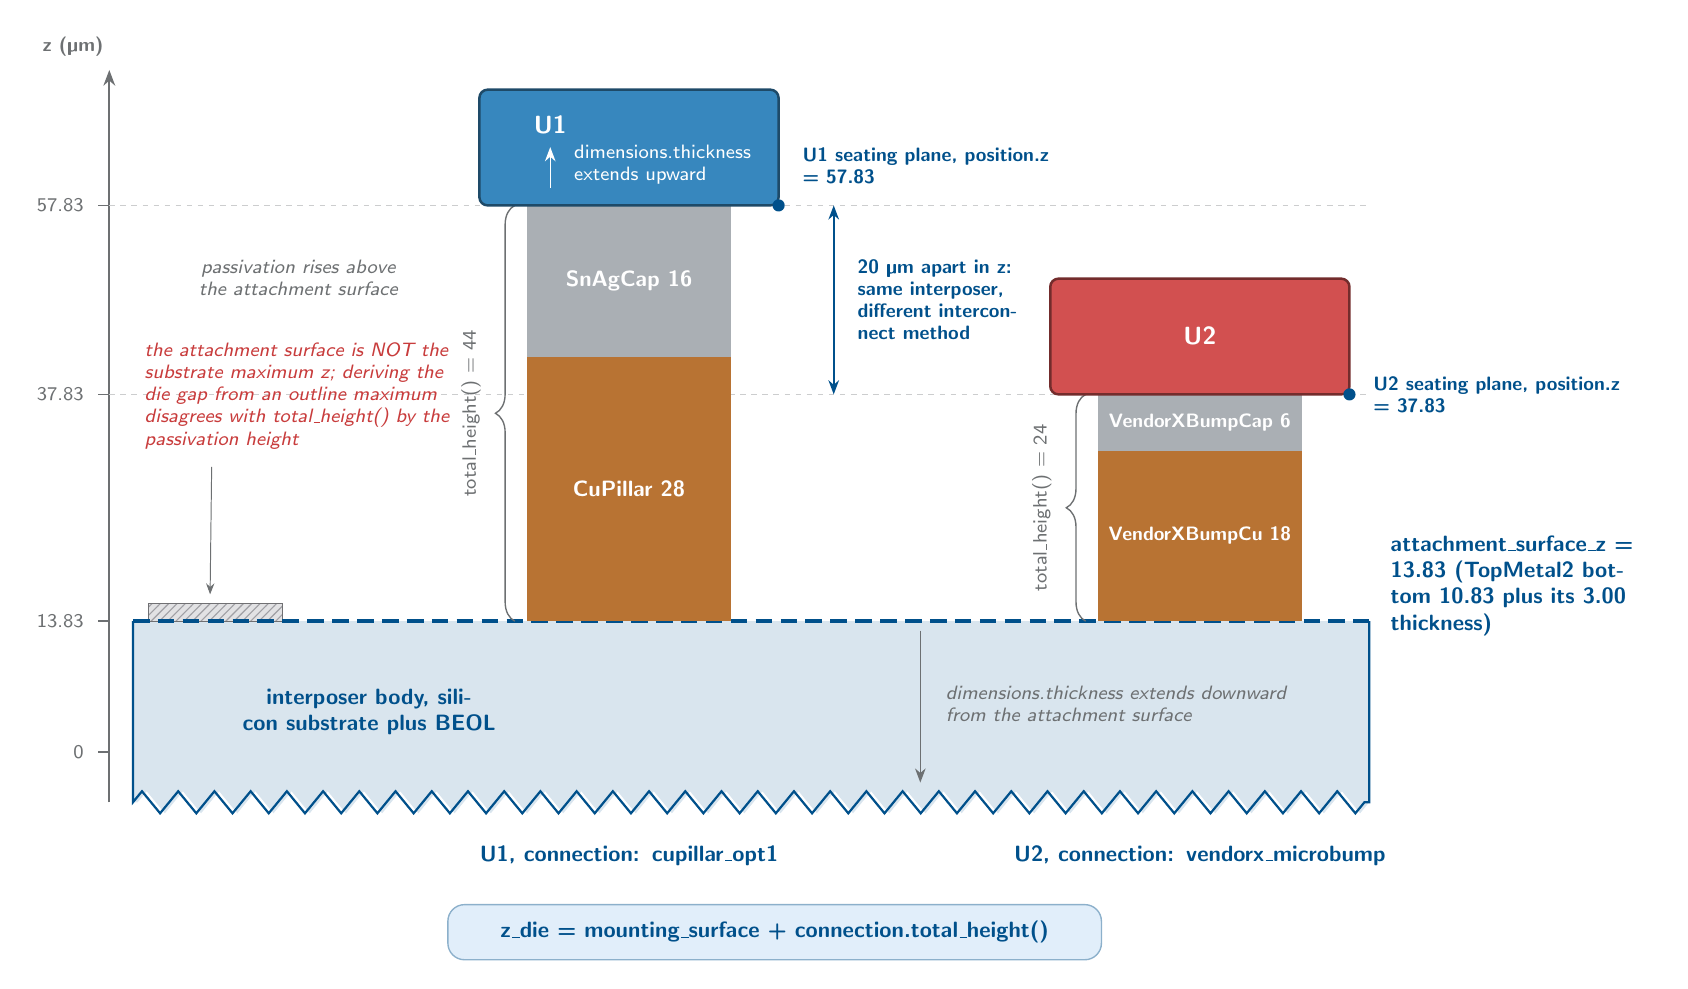
\begin{tikzpicture}[
    adklayerlbl/.style={font=\sffamily\footnotesize\bfseries, text=white,
                        align=center},
    adksmalllbl/.style={font=\sffamily\scriptsize\bfseries, text=white,
                        align=center},
    adkbodylbl/.style={font=\sffamily\footnotesize\bfseries, text=IHPfg,
                       align=center},
    adknote/.style={font=\sffamily\scriptsize\itshape, text=IHPaccent,
                    align=left},
    adknotec/.style={font=\sffamily\scriptsize\itshape, text=IHPaccent,
                     align=center},
    adkwarn/.style={font=\sffamily\scriptsize\itshape, text=cWarn,
                    align=left},
    adkaxis/.style={line width=0.6pt, color=IHPaccent},
    adkaxislbl/.style={font=\sffamily\scriptsize, text=IHPaccent,
                       anchor=east},
    adkguide/.style={line width=0.35pt, color=IHPaccent!35, dash pattern=on 2pt off 2pt},
    adkarrow/.style={-{Stealth[length=1.8mm]}, line width=0.5pt,
                     color=IHPaccent},
    adkdblarrow/.style={{Stealth[length=1.8mm]}-{Stealth[length=1.8mm]},
                        line width=0.6pt, color=IHPfg},
    adkleader/.style={-{Stealth[length=1.4mm]}, line width=0.35pt,
                      color=IHPaccent},
    adkbrace/.style={decorate, decoration={brace, amplitude=7pt},
                     line width=0.5pt, color=IHPaccent},
    adkbracelbl/.style={font=\sffamily\scriptsize, text=IHPaccent}
]

% ---------------------------------------------------------------------------
% Geometry. y = (z - 13.83) * 0.12 cm, true scale everywhere above the break.
% ---------------------------------------------------------------------------
\def\yattach{0}        % z = 13.83  attachment surface
\def\yutwo{2.88}       % z = 37.83  U2 seating plane  (13.83 + 24)
\def\yuone{5.28}       % z = 57.83  U1 seating plane  (13.83 + 44)
\def\yzero{-1.66}      % z =  0.00  silicon surface
\def\ybreak{-2.30}     % break line, inside the substrate
\def\xleft{0.30}
\def\xright{16.00}

% --- interposer body, top face on the attachment surface, broken at bottom ---
% Filled first, then outlined on three sides only, so the dashed attachment
% surface remains the sole line along the top face.
\fill[cInterposer!15]
    (\xleft, \yattach) -- (\xright, \yattach) -- (\xright, \ybreak)
    decorate[decoration={zigzag, amplitude=1.4mm, segment length=4.6mm}]
        { -- (\xleft, \ybreak) }
    -- cycle;
\draw[cInterposer, line width=0.8pt]
    (\xleft, \yattach) -- (\xleft, \ybreak)
    decorate[decoration={zigzag, amplitude=1.4mm, segment length=4.6mm}]
        { -- (\xright, \ybreak) }
    -- (\xright, \yattach);

\node[adkbodylbl, text width=5.0cm] at (3.30, -1.15)
    {interposer body, silicon substrate plus BEOL};

% thickness grows downward from the attachment surface
\draw[adkarrow] (10.30, -0.12) -- (10.30, -2.05);
\node[adknote, anchor=west, text width=4.9cm] at (10.50, -1.05)
    {dimensions.thickness extends downward from the attachment surface};

% ---------------------------------------------------------------------------
% z axis
% ---------------------------------------------------------------------------
\draw[adkaxis, -{Stealth[length=2mm]}] (0, \ybreak) -- (0, 7.00);
\node[font=\sffamily\scriptsize\bfseries, text=IHPaccent, anchor=south east]
    at (0.05, 7.05) {z (\textmu m)};

\foreach \yy/\lbl in {\yzero/0, \yattach/13.83, \yutwo/37.83, \yuone/57.83} {
    \draw[adkaxis] (-0.14, \yy) -- (0, \yy);
    \node[adkaxislbl] at (-0.20, \yy) {\lbl};
}

% faint guides across the drawing
\foreach \yy in {\yutwo, \yuone} {
    \draw[adkguide] (0, \yy) -- (\xright, \yy);
}

% ---------------------------------------------------------------------------
% passivation, sitting on the interposer top face and rising above it
% ---------------------------------------------------------------------------
\fill[cPass!30] (0.50, \yattach) rectangle (2.20, 0.228);
\fill[pattern=north east lines, pattern color=cPass]
    (0.50, \yattach) rectangle (2.20, 0.228);
\draw[cPass!70!black, line width=0.4pt]
    (0.50, \yattach) rectangle (2.20, 0.228);

\node[adknotec, text width=3.9cm] at (2.40, 4.36)
    {passivation rises above the attachment surface};

% the trap this figure exists for
\node[adkwarn, text width=3.9cm] at (2.40, 2.86)
    {the attachment surface is NOT the substrate maximum z; deriving the die
     gap from an outline maximum disagrees with total\_height() by the
     passivation height};

\draw[adkleader] (1.30, 1.96) -- (1.28, 0.34);

% ---------------------------------------------------------------------------
% the attachment surface itself
% ---------------------------------------------------------------------------
\draw[IHPfg, line width=1.3pt, dash pattern=on 6pt off 3pt]
    (\xleft, \yattach) -- (\xright, \yattach);
\node[font=\sffamily\footnotesize\bfseries, text=IHPfg, anchor=west,
      text width=3.3cm, align=left] at (16.15, 0.45)
    {attachment\_surface\_z = 13.83 (TopMetal2 bottom 10.83 plus its 3.00 thickness)};

% ---------------------------------------------------------------------------
% U1, cupillar_opt1: CuPillar 28 + SnAgCap 16 = 44
% ---------------------------------------------------------------------------
\def\uonel{5.30}
\def\uoner{7.90}
\fill[cCuPillar] (\uonel, \yattach) rectangle (\uoner, 3.36);
\node[adklayerlbl] at (6.60, 1.68) {CuPillar 28};

\fill[cSnAg] (\uonel, 3.36) rectangle (\uoner, \yuone);
\node[adklayerlbl] at (6.60, 4.32) {SnAgCap 16};

\draw[adkbrace] (5.15, \yattach) -- (5.15, \yuone);
\node[adkbracelbl, rotate=90, anchor=south] at (4.84, 2.64)
    {total\_height() = 44};

% U1 die block, bottom face exactly on the 57.83 guide
\fill[cDieA, draw=cDieA!55!black, line width=0.9pt, rounded corners=3pt]
    (4.70, \yuone) rectangle (8.50, 6.75);
\node[font=\sffamily\small\bfseries, text=white] at (5.60, 6.30) {U1};
\draw[-{Stealth[length=1.8mm]}, line width=0.5pt, color=white]
    (5.60, 5.50) -- (5.60, 6.02);
\node[font=\sffamily\scriptsize, text=white, anchor=west, text width=2.45cm]
    at (5.78, 5.80) {dimensions.thickness extends upward};

\fill[IHPfg] (8.50, \yuone) circle (2.2pt);
\node[font=\sffamily\scriptsize\bfseries, text=IHPfg, anchor=west,
      text width=3.4cm, align=left] at (8.68, 5.78)
    {U1 seating plane, position.z = 57.83};

\node[adkbodylbl, text width=4.0cm] at (6.60, -2.98)
    {U1, connection: cupillar\_opt1};

% ---------------------------------------------------------------------------
% U2, vendorx_microbump: VendorXBumpCu 18 + VendorXBumpCap 6 = 24
% ---------------------------------------------------------------------------
\def\utwol{12.55}
\def\utwor{15.15}
\fill[cCuPillar] (\utwol, \yattach) rectangle (\utwor, 2.16);
\node[adksmalllbl] at (13.85, 1.08) {VendorXBumpCu 18};

\fill[cSnAg] (\utwol, 2.16) rectangle (\utwor, \yutwo);
\node[adksmalllbl] at (13.85, 2.52) {VendorXBumpCap 6};

\draw[adkbrace] (12.40, \yattach) -- (12.40, \yutwo);
\node[adkbracelbl, rotate=90, anchor=south] at (12.09, 1.44)
    {total\_height() = 24};

% U2 die block, bottom face exactly on the 37.83 guide
\fill[cDieB, draw=cDieB!55!black, line width=0.9pt, rounded corners=3pt]
    (11.95, \yutwo) rectangle (15.75, 4.35);
\node[font=\sffamily\small\bfseries, text=white] at (13.85, 3.62) {U2};

\fill[IHPfg] (15.75, \yutwo) circle (2.2pt);
\node[font=\sffamily\scriptsize\bfseries, text=IHPfg, anchor=west,
      text width=3.3cm, align=left] at (15.93, 2.88)
    {U2 seating plane, position.z = 37.83};

\node[adkbodylbl, text width=5.2cm] at (13.85, -2.98)
    {U2, connection: vendorx\_microbump};

% ---------------------------------------------------------------------------
% the 20 um difference between the two seating planes
% ---------------------------------------------------------------------------
\draw[adkdblarrow] (9.20, \yutwo) -- (9.20, \yuone);
\node[font=\sffamily\scriptsize\bfseries, text=IHPfg, anchor=west,
      text width=2.2cm, align=left] at (9.38, 4.08)
    {20 \textmu m apart in z: same interposer, different interconnect method};

% ---------------------------------------------------------------------------
% formula banner
% ---------------------------------------------------------------------------
\filldraw[IHPlight, draw=IHPfg!45, line width=0.5pt, rounded corners=6pt]
    (4.30, -4.30) rectangle (12.60, -3.60);
\node[font=\sffamily\footnotesize\bfseries, text=IHPfg] at (8.45, -3.95)
    {z\_die = mounting\_surface + connection.total\_height()};

\end{tikzpicture}
\end{document}
